\documentclass[tikz,border=12pt]{standalone}
\usepackage{fontspec}
\setmainfont{Segoe UI}
\usepackage{amsmath,amssymb}
\usepackage{tikz}

\usetikzlibrary{calc,arrows.meta}

\begin{document}
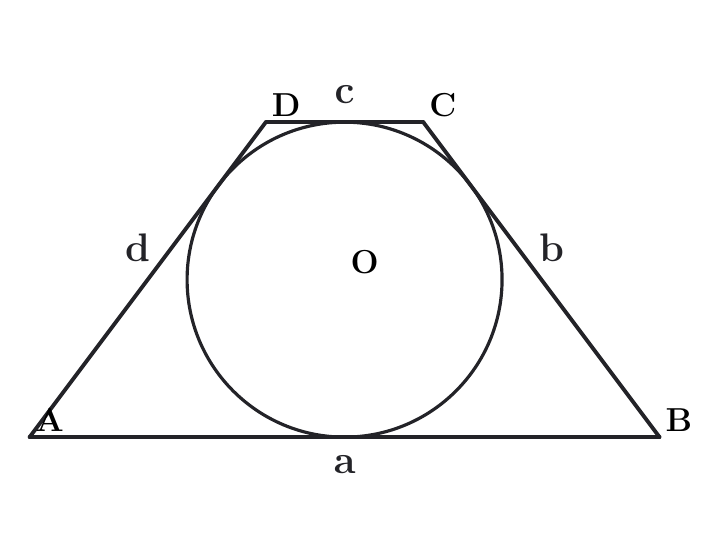
\begin{tikzpicture}[x=1.0000cm,y=1cm,line cap=round,line join=round]
\definecolor{linec0}{RGB}{35,35,40}
\definecolor{linec1}{RGB}{35,35,40}
\definecolor{linec2}{RGB}{35,35,40}
\definecolor{linec3}{RGB}{35,35,40}
\definecolor{linec4}{RGB}{35,35,40}
\definecolor{linec5}{RGB}{35,35,40}
\definecolor{edgecol}{RGB}{35,35,40}
\definecolor{hicol}{RGB}{35,35,40}
\definecolor{angcol}{RGB}{35,35,40}
\coordinate (A) at (0.0000,0.0000);
\coordinate (B) at (8.0000,0.0000);
\coordinate (C) at (5.0000,4.0000);
\coordinate (D) at (3.0000,4.0000);
\coordinate (O) at (4.0000,2.0000);
\coordinate (X) at (4.0000,0.0000);
\draw[line width=1.4pt,color={rgb,255:red,35;green,35;blue,40}] (A) -- (B);
\draw[line width=1.4pt,color={rgb,255:red,35;green,35;blue,40}] (B) -- (C);
\draw[line width=1.4pt,color={rgb,255:red,35;green,35;blue,40}] (C) -- (D);
\draw[line width=1.4pt,color={rgb,255:red,35;green,35;blue,40}] (D) -- (A);
\draw[edgecol,line width=1.15pt] (O) circle [x radius=2.0000, y radius=2.0000];
\path (0.800,-1.200) rectangle (7.200,5.200);
\node[font=\bfseries\Large,text={rgb,255:red,35;green,35;blue,40}] at (4.000,-0.350) {a};
\node[font=\bfseries\Large,text={rgb,255:red,35;green,35;blue,40}] at (6.630,2.410) {b};
\node[font=\bfseries\Large,text={rgb,255:red,35;green,35;blue,40}] at (4.000,4.350) {c};
\node[font=\bfseries\Large,text={rgb,255:red,35;green,35;blue,40}] at (1.370,2.410) {d};
\node[font=\bfseries\large,inner sep=2pt,anchor=south west] at (0.000,0.000) {A};
\node[font=\bfseries\large,inner sep=2pt,anchor=south west] at (8.000,0.000) {B};
\node[font=\bfseries\large,inner sep=2pt,anchor=south west] at (5.000,4.000) {C};
\node[font=\bfseries\large,inner sep=2pt,anchor=south west] at (3.000,4.000) {D};
\node[font=\bfseries\large,inner sep=2pt,anchor=south west] at (4.000,2.000) {O};
\end{tikzpicture}
\end{document}
